\documentclass[11pt]{article}
\usepackage[top=1.00in, bottom=1.0in, left=1in, right=1in]{geometry}
\renewcommand{\baselinestretch}{1.1}
\usepackage{graphicx}
\usepackage{natbib}
\usepackage{amsmath}
\usepackage{parskip}
\usepackage{hyperref}
\usepackage{gensymb}

\def\labelitemi{--}

\usepackage{fancyhdr}
\pagestyle{fancy}
\fancyhead[LO]{}
\fancyhead[RO]{}

\begin{document}
\bibliographystyle{/Users/Lizzie/Documents/EndnoteRelated/Bibtex/styles/besjournals}
\renewcommand{\refname}{\CHead{}}


\title{How to fit Bayesian models and influence people \emph{or}\\
How to do Bayesian model fitting in ecology \emph{or}\\
The best way to be a Bayesian in ecology today}
\date{\today}
\author{EM Wolkovich and WD Pearse and M Betancourt? and TJ Davies?}
\maketitle

\abstract{Improvements in algorithms and computational speed have heralded a new a era of Bayesian model fitting. Models are easier to fit, faster to run, and more flexible to fit, making them ideal for many of the complexities of ecological sampling designs. This has opened up Bayesian approaches to a new world of users, but how best to start using and implementing Bayesian approaches in ecology is still somewhere between old rules and methods and the new school where Bayesian approaches also include a specific workflow of not just how to do stats, but how to do science. Here we review a simple form of a Bayesian workflow that integrates mechanistic and statistical models with a computational toolkit that we argue could accelerate ecological science. [Maybe along the way we highlight common practices in ecology that are stupid as all tomorrow---as our approach makes clear---and outline best practices for jumping into the wonderful surf of the happy Bayesian ocean.]} 

\section{Main text}

Recent years have seen the explosion of Bayesian models across fields (CITES), including ecology. This change comes in part from increased computational power, but more from new algorithms (e.g., Hamiltonian Monte Carlo) that have made models faster and arguably easier to fit. Capitalizing on these advances \textsf{R} packages such as \textsf{brms} have seen much wider use than the previous generation of packages that streamlined fitting a set of pre-determined models using Bayesian approaches (\eg \textsf{MCMCglmm}. Bayesian approaches, long heralded as more powerful, flexible and especially adept at capturing the multiple levels of variance in ecological data, seem poised to help ecology as a discipline advance in leaps and bounds.

Ecology itself seems poised to leap out of the jungle and land into the role society is asking of it as growing global challenges demand more predictive models of how communities and ecosystems will shift with climate change, habitat degradation and all that jazz. Ecology is now three decades on after the start of the synthesis movement, which required more advanced statistical and computational approaches of ecology to test fundamental theory across systems (CITES). Early concerns have given way to a widespread appreciation of the value of these new approaches, alongside a resounding fervor over `natural history.' At the same time, the growing anthropogenic challenges have increased the need for predictive models and forecasts from ecologists. 

The result is that the average ecologist today has a diversified skillset compared to that of decades ago. Ecology has long been a field with deep statistical training, but in many ways the modern ecologist is now also expected to be computational---able to handle large datasets, produce repeatable workflows and help translate models into forecasts for planning. Many  ecologists now bridge field and computational methods. As such, the rise of Bayesian approaches is especially timely for ecology. % The average modern ecologist is computational, but often grounded in the natural history of a particular system (err, maybe, on both these accounts, but whatever).

Bayesian approaches are in no way new to ecology, as they have long been used in certain subdisciplines related to estimating population sizes of things people want to eat or manage. For example, wildlife biology widely uses mark-recapture data and associated models to estimate population sizes; these methods almost always use Hidden Markov models (HMM), which can rarely be fit without Bayesian methods (CITES). Similarly, fisheries biology has tended towards more complex models---such as state-space models---to estimate fish stocks, which are similarly easiest to fit with Bayesian approaches (CITES). For decades, Bayesian training in ecology has focused on these aims, but as data and methods change, so has how ecologists are using Bayesian models. 

Today, as large-scale ecological data becomes available for more diverse systems and for questions addressing other aims, more ecologists are using Bayesian models in new ways. Yet, at the same time, training in statistics and in Bayesian modeling in particular may struggle to keep pace. Bayesian approaches provide a pathway to powerful models that can transform how we understand our systems, but they can also lead to pitfalls most ecologists are not trained to notice or deal with. These pitfalls can be avoided by approaching Bayesian analyses through specific workflows (CITES), which themselves are built on a process of how to do not just stats, but science. Here we describe a broadly generalizable workflow for Bayesian analysis and show how it can revolutionize training in ecology by integrating more model building and model understanding. Once you start doing this workflow, your scientific life will never be the same. 
%  allow fitting complex models without much influence of the data fed into the model. 

\subsection{Box by WPD with 3 paragraph explanation of Bayes}

Someone with the initials WPD will hopefully write this. 

\subsection{A brief overview of the benefits---and pitfalls---of Bayesian models} 

Bayesian models have many benefits, but an often-mentioned one is that `you can fit any model you want.' While this is not entirely true (CITES), compared to the models ecologists can fit in popular modeling packages (\eg \testsf{lme4}) Bayesian modeling options can feel limitless. As long as you can write the out the likelihood of your desired model and assign priors to all parameters, you can generally `fit' any model. This includes non-linear ones, non-Gaussian families (\eg Poisson, beta or combinations thereof such as hurdle models), hierarchical designs and any combination of these, as well as `joint' models where parameters estimated in one equation appear in another, thus carrying through estimated uncertainty. Such flexibility is incredibly powerful in ecology where data are often influenced by complex spatial or temporal patterns, non-linear processes are widespread and common data types are non-Gaussian (\eg counts, percent cover etc.). 

Fitting a bespoke model to your data and question frees scientists to estimate useful parameters---effectively, a way to get the numbers we often really want but don't have access to. Thus, instead of reporting a treatment's p-value and accompanying F statistic and degrees of freedom, models can be designed to estimate and report effects per \degree C of warming or at what level non-linearities due to high temperature begin---always with estimated uncertainty. While replication crises in other fields, driven in part by a overly zealous focus on p-values (CITES), and the rise of meta-analyses in ecology (CITES) have led to a somewhat greater focus on `effect sizes' in ecology (often used to refer to very specific unitless statistics, such as Cohen's $d$), bespoke models take this to a new level. Researchers can easily estimate comparable effect sizes from z-scored data, alongside estimates in meaningful natural units, such as per \degree C of warming or per hectare of habitat lost. 

But this valuable flexibility is also one of the greatest pitfalls of Bayesian models You can fit almost whatever you want, but critical parts of your model might be almost entirely unimpacted by your data. And in ecological model fitting, we're most often interested in parameter estimates strongly informed by our data. 

This `pitfall' of Bayesian is not new, nor unique to ecology---though the complexity of ecological data and processes may make it especially pernicious in ecology---and decades of statistical research has aimed to develop best practices when using Bayesian models to avoid this. These best practices generally center around a specific workflow; a variety of which can be found in exquisite detail elsewhere (CITES). We do not aim to repeat those here, but instead to provide you with a highly simplified but powerful workflow we believe when applied to Bayesian modeling in ecology could greatly accelerate progress. % This is a short overview of a much deeper topic. See \href{https://www.nature.com/articles/s43586-020-00001-2}{Bayesian statistics and modelling} for a little more depth, including how to develop priors and your basic model formulation.\\

\subsection{Our simple Bayesian workflow}

We outline a basic Bayesian workflow below that includes the major steps for Bayesian model fitting. Many steps should be familiar to statistical ecologists, but are often overlooked, whereas other steps may appear particular to Bayesian (\eg prior predictive checks), but are actually useful for anyone---using Bayesian models or not---to challenge their models of how the world works, and learn from them. 

We assume a user of \textsf{Stan}, a relatively new probabalistic programming language, that interfaces with \textsf{R, Python, Julia} (and more) to write bespoke Bayesian models and underpins the \textsf{R} packages \textsf{brms} and \textsf{rstanarm}, which fit a suite of specific (pre-defined) models. We focus on \textsf{Stan} as its MCMC algorithm (a variant of Hamiltonian Monte Carlo, HMC) is fast and produces specific output to warn of model fit issues (i.e., divergent transitions) in a way other MCMC algorithms do not (\eg Metropolis or GIBBS), but the basic workflow should apply to diverse implementations of Bayesian modeling. \\

{\Large \bf Start here Lizzie!} \\

\emph{Note that you might need to start simple and build up to get all these steps to work, but this is my recommended approach to the basic workflow.}

\begin{enumerate}
\item Check your code. Write down your model -- I recommend as basic math, then write it in \verb|Stan| and simulate one set of test data (often in \verb|R|). I recommend you do this first because it will flesh out any issues in your simulated data (\verb|R|) code, which you need right away (but you don't need the \verb|Stan| code until step 3).
\begin{enumerate}
\item Write your \verb|Stan| code.
\item In \verb|R|, write simulated data where you {\bf write out all your parameters}, write $x$ and generate $y$ from your model. So, if I am doing simple regression ($y=mx+b$, with error $\epsilon$) then I would have to assign values to $m, b$ and $\epsilon$ and I would generate a vector of $x$ values, then I would simulate $y$ from those values.
\item Run your \verb|Stan| code on your simulated data. Check that your \verb|Stan| code returns your model parameters, if not, check your code, set your error lower and/or sample size higher. Keep checking until your \verb|Stan| output matches your parameters (note check your \verb|Stan| code and your simulated data code) and you trust both.
\end{enumerate}
\item Prior predictive checks: Check yo' priors.
\begin{enumerate}
\item Take your aforementioned \verb|R| code and set up priors for each parameter (e.g., distributions for $m, b, \epsilon$). {\bf In contrast to above, where you just set each parameter to one value, here you you want to draw multiple values for each parameter and visually check the output.} 
\item How do I check the output? Just like posterior predictive checks, this is up to you! At a minimum I recommend thinking of plots you will make with your model in the end (for publications) and plotting that given different prior values.
\item Your goal here is to check that your priors are reasonable, if they are not, adjust them. 
\item Unlike in Step 1, you do {\bf not} need to run \verb|Stan|---you have your parameters so you can just simulate data from them, and then plot, examine etc.. No \verb|Stan| at this step. 
\end{enumerate}
\item Now you can run your model on your real data!
\begin{enumerate}
\item Check the output, if you have divergent transitions, you need to re-parameterize your model (may tried a non-centered model or such).
\item I recommend ShinyStan here.
\end{enumerate}
\item Posterior predictive checks: How good or bad does your model do compared to your data?
\begin{enumerate}
\item Grab the parameter values from your fitted \verb|Stan| model. In posterior predictive checks \emph{these are the parameter values you use to simulate new data.}  
\item You can adapt your \verb|R| code for simulating data above, but use your estimated parameters from your fitted model. 
\item What should I look at? Ah, just like in prior predictive checks, you need to decide. Classic things are to look at the mean of 100 or so simulations of new data you generate versus your {\bf real} data. Also try the SD. Plot things! Look at the distribution. If you use the generated quantities block in \verb|Stan| ShinyStan will automatically generate a few plots but think hard about more.
\item When does this get hard? In hierarchical models (and other models with hyperparameters) as you have multiple levels you can generate---you can use \emph{your estimated parameters from your fitted model at all levels or generate your lower-level parameters} (for example, you can generate species means using your species $\mu$ and $\sigma$). You have to think about what you want your model to predict.
\item See how it is---do you see obvious problems caused by the distribution you selected or a grouping factor you're missing? If so, add it. And go back to Step 1. 
\item (No \verb|Stan| at this step.)
\end{enumerate}
\end{enumerate}

{\bf Benefits of this workflow}

\begin{enumerate}
\item More fully integrates the mathematical model to statistical part of Bayesian -- you have to write the model with test data before you fit to your data
\item Both the test data writing and the posterior predictive checks dive you deep into understanding your mechanistic-statistical model and that, in our experience, gives you WAY more insights and ideas into your biological model and---wait for it---your biological system!
\end{enumerate}


\subsection{Surprising things that happened to us that may happen to you if you follow this workflow}

\begin{enumerate}
\item We got deeply in touch with the term {\bf nonidentifiability} and how it can happen (model nonidentifiability and data + model nonidentifiability) ... now that you can fit any model you want, you see this happen (before, a Hessian problem may have stood in your way sometimes for these models, but also sometimes for perfectly good models)
\item Simplify! Simplify! Simplify! Once you do the workflow, you may end up like us: fitting fewer levels in your mixed effects models, fitting fewer interactions.
\item Started comparing actual numbers, not p-values
\item Don't cram the world into your model ... in contrast, value of the posterior for manipulation. 
\item Plotting: The whole big wide world between plotting your raw data and plotting you model ... Plotting `partials' of your model (remove the site effects, for example).
\end{enumerate}

\subsection{Challenges of the workflow compared to how we traditionally train ecologists (or, how this will reshape ecological training)}

\begin{enumerate}
\item Good stats workflows bleed into what we expect of theoretical ecologists (and yet we act like non-theory folks should be trained differently). 
\item Theory = simpler models = outcome of a good Bayesian workflow (often)
\end{enumerate}

Moving away from old school Bayesian and into the light -- Read this section to the tune of `Let it go' from \emph{Frozen} 
\begin{enumerate}
\item Everyone can be a Bayesian, not just wildlife and fisheries biologists (aka HMM and state-space people)
\item Please, stop going on and on about priors. 
\item Conjugate priors as the crystal deodorant of priors (check Dan Simpson quote)
\item Let go of `random' versus fixed effects ideas
\item Let go of p-values and embrace numbers with units! (\href{https://www.youtube.com/watch?v=c3hxhv0lpI0}{`I am arbitrary but my story is often told ... '}
\end{enumerate}

\subsection{Conclusions}
\begin{enumerate}
\item Ecologists cannot simulate their stats (or simple systems for that matter). Evolutionary biologists can. (And the field is better for it.)
\item Maybe hint at that you need these skills (and unit testing) given rise of AI?
\end{enumerate}

{\bf Take home messages (maybe)}
\begin{enumerate}
\item You should not fit a model you cannot simulate
\item Fit simpler models
\item Know your nonidentifiability
\end{enumerate}

\section{Figures}

\begin{figure}[ht]
\centering
\noindent 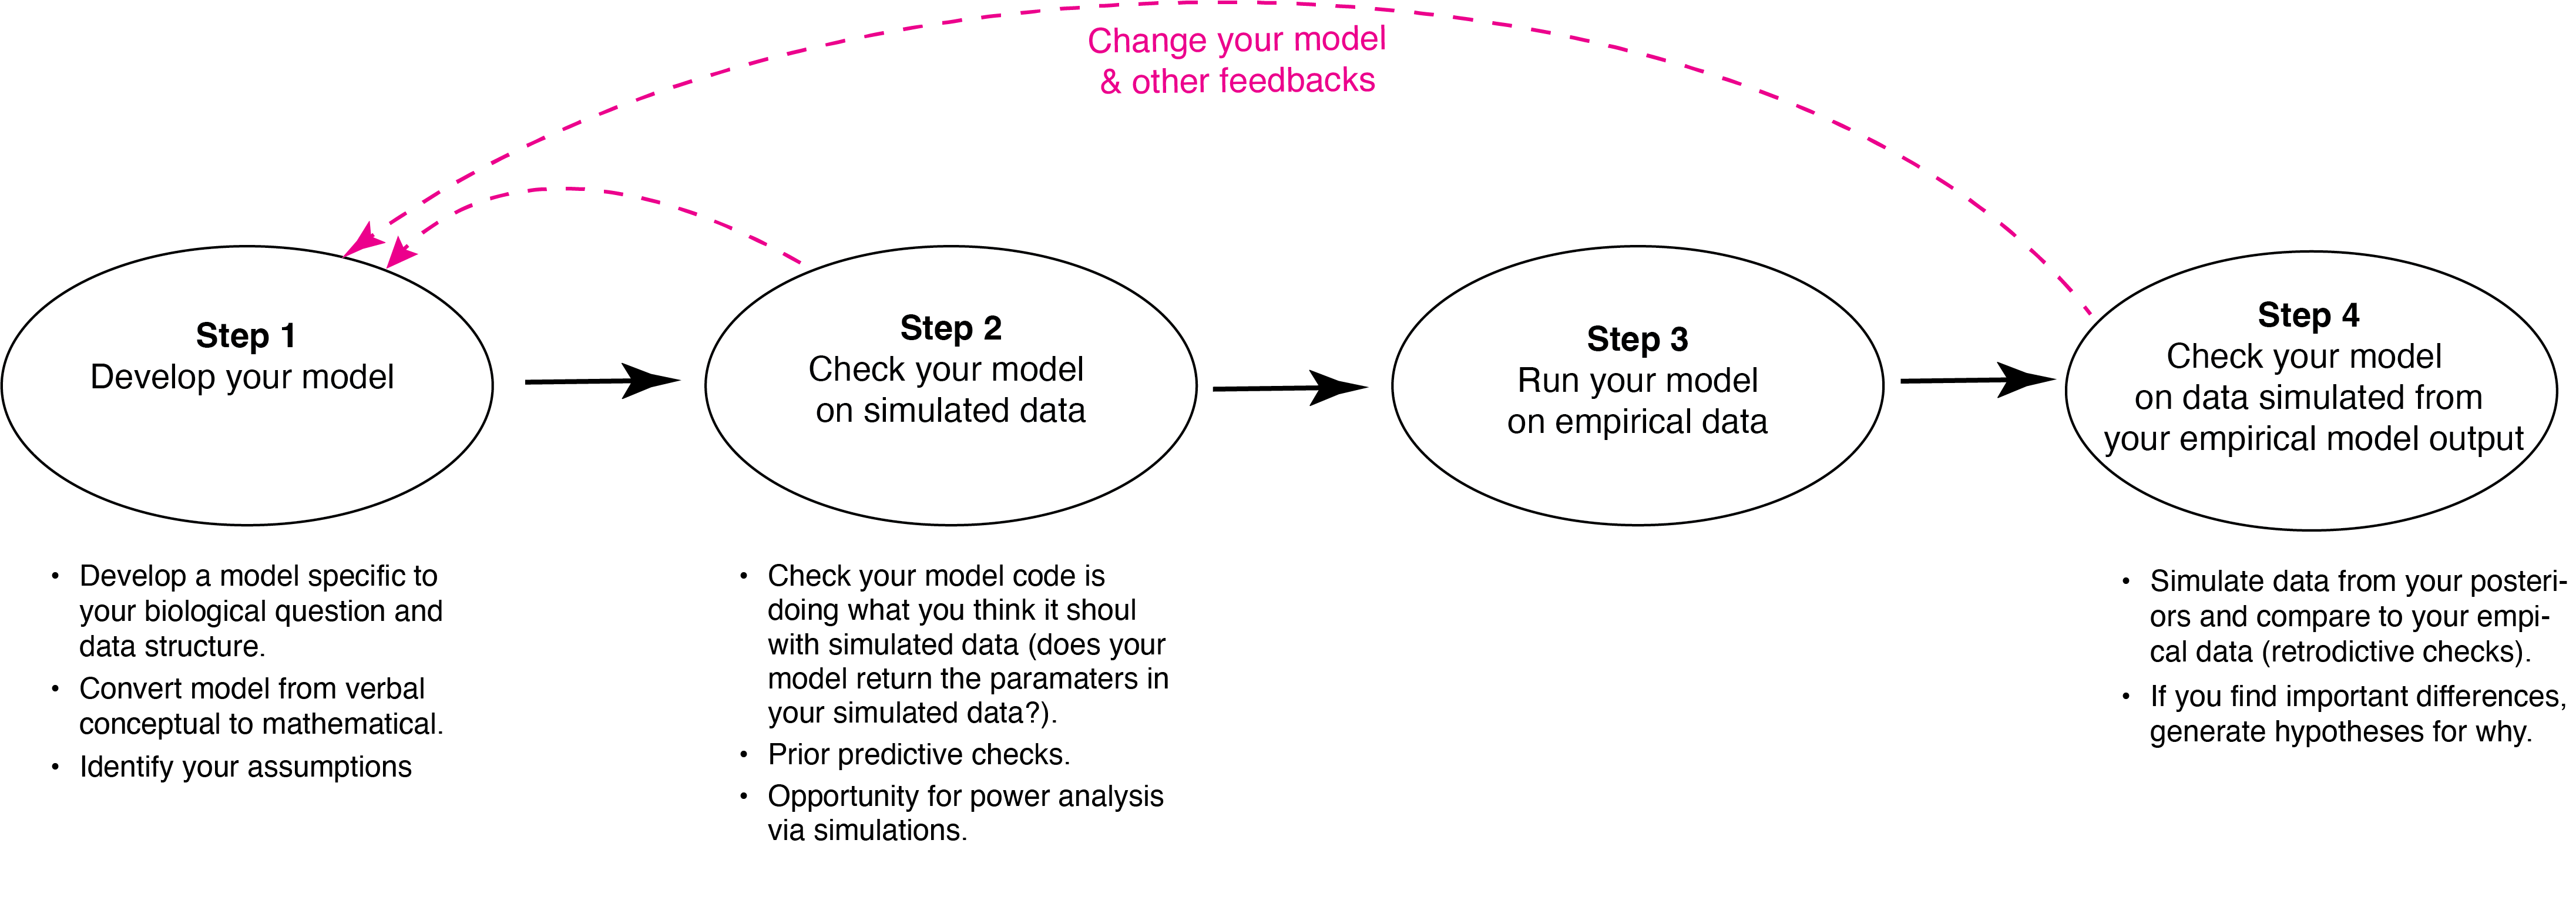
\includegraphics[width=0.7\textwidth]{figures/workflow.png}
\caption{Simple workflow.}
\label{fig:workflow}
\end{figure}

\begin{figure}[ht]
\centering
\noindent 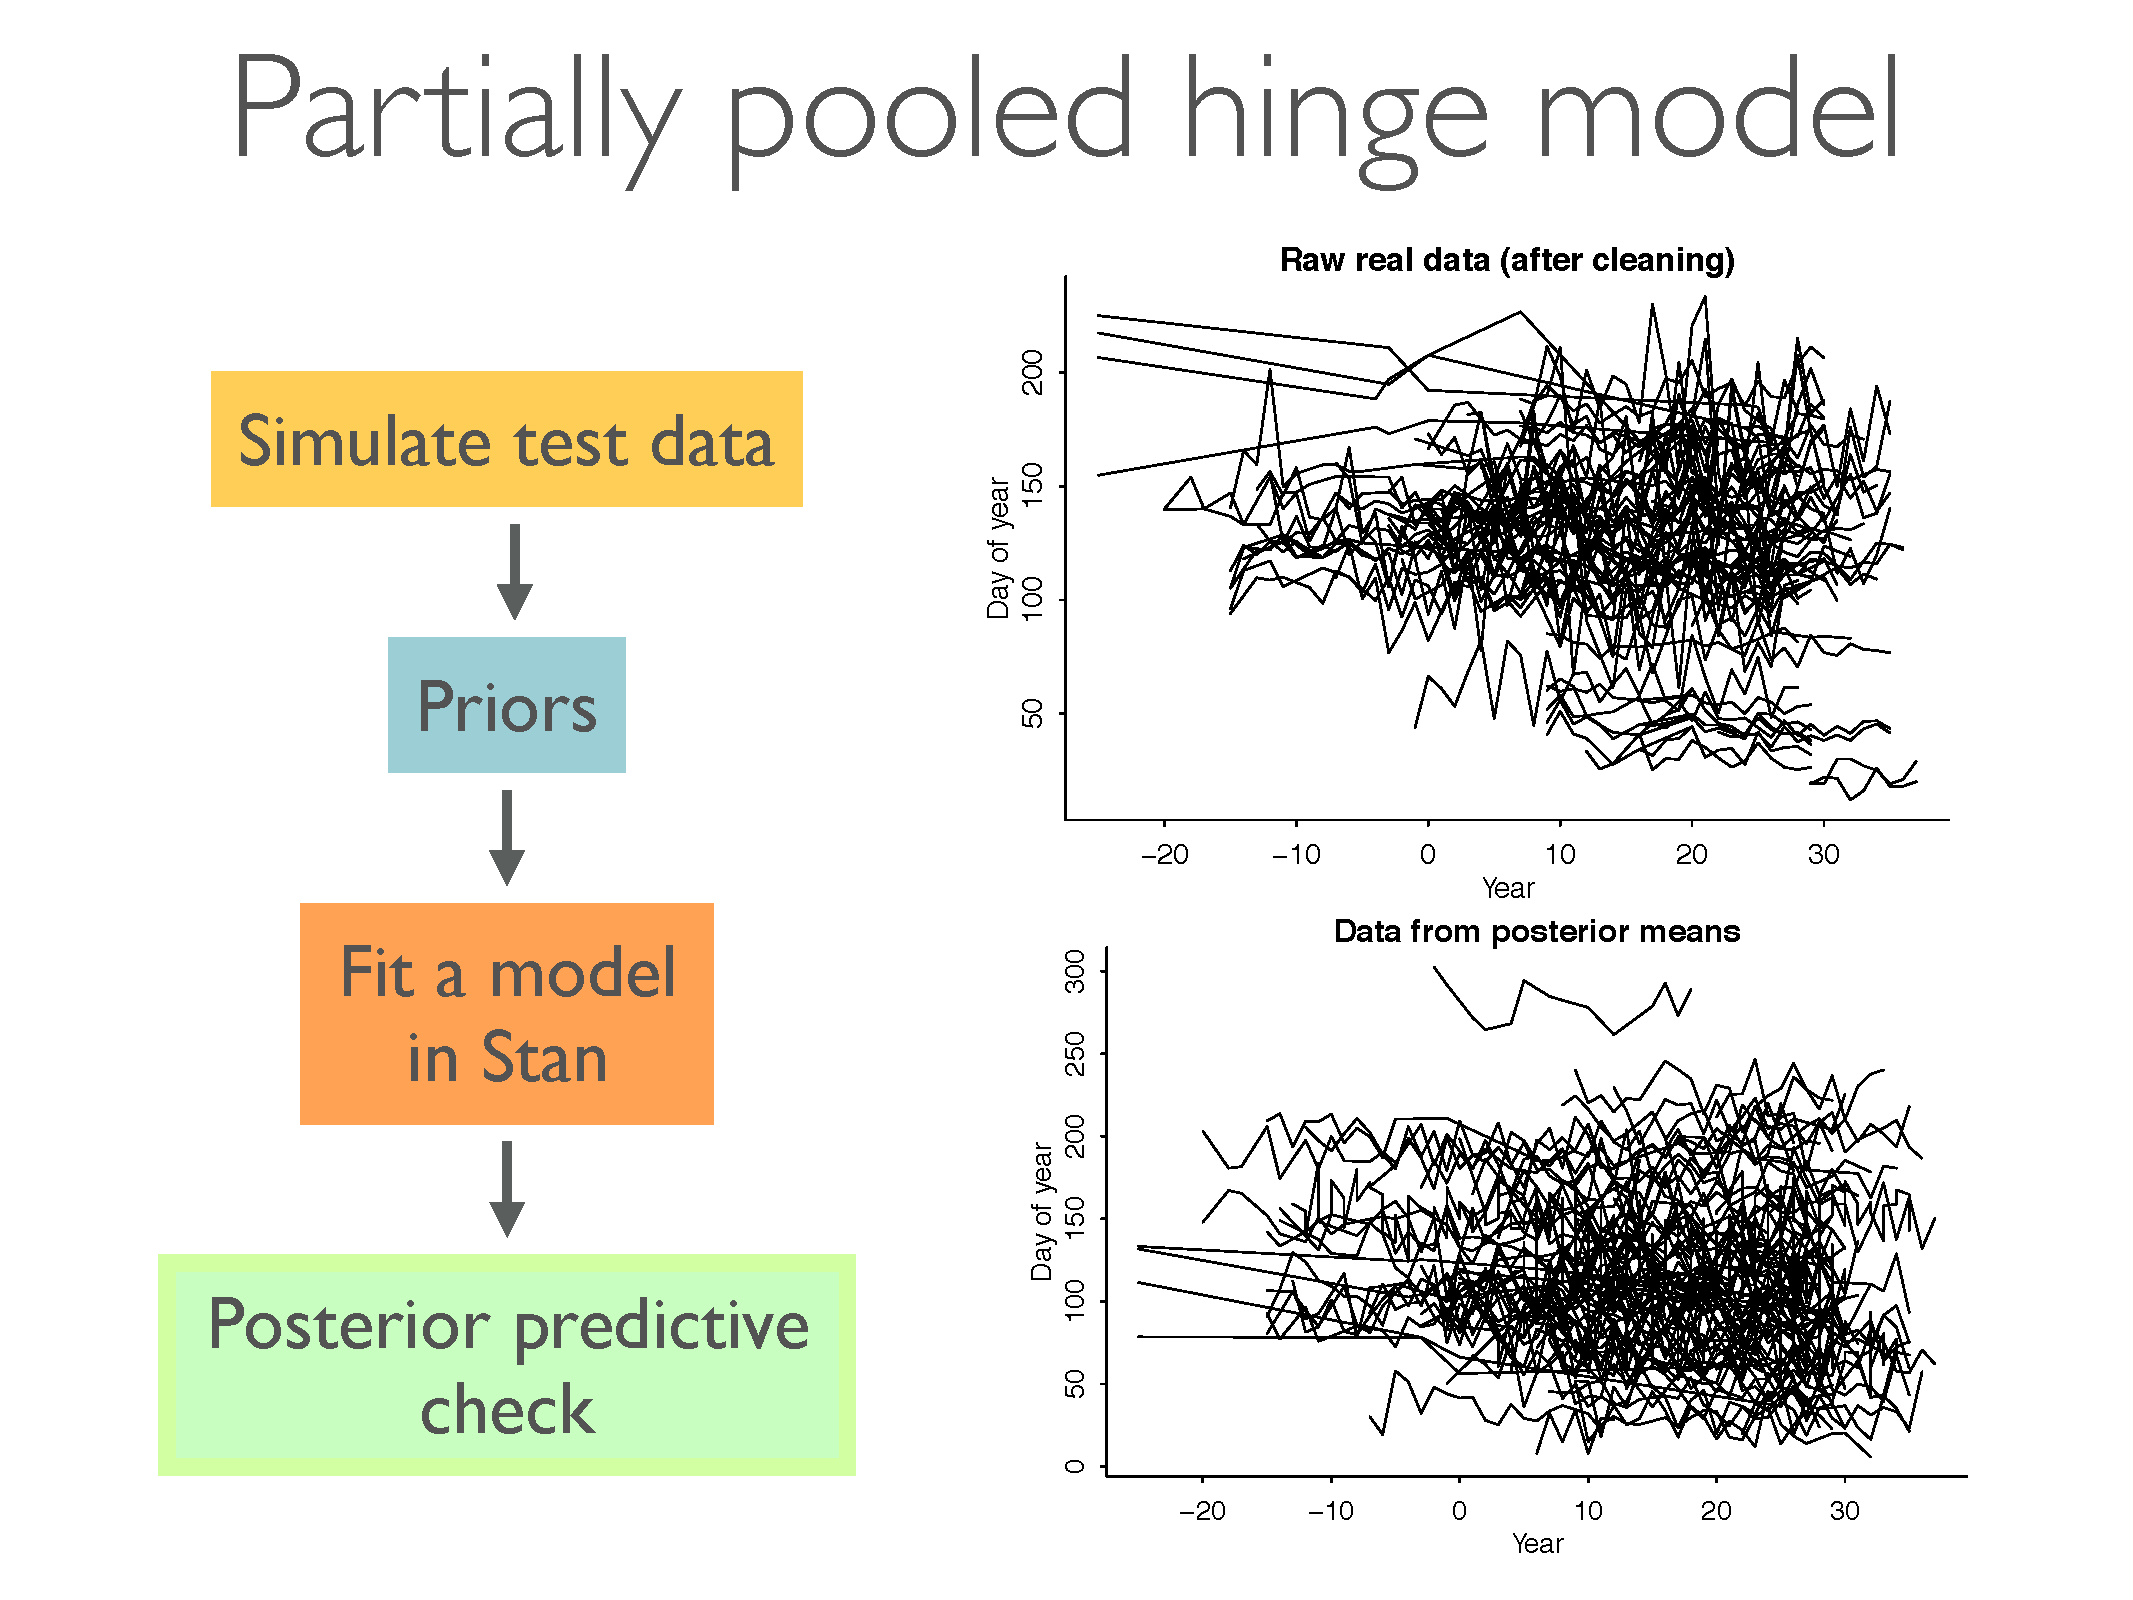
\includegraphics[width=0.8\textwidth]{figures/Pages_from_generablestannyc.pdf}
\caption{Reminder to Lizzie of a retrodictive check we could include.}
\label{fig:retrodictivecheck}
\end{figure}

\end{document}